\documentclass[main.tex]{subfiles}
\newcommand{\D}{\mathcal{D}}
\newcommand{\Kc}{\mathcal{K}}
\newcommand{\Lc}{\mathcal{L}}
\begin{document}
\section{Trajectoire}

Dans le cas linéaire, la trajectoire est la solution au système $\dot{x}=Ax$ avec $x(0)=x_0$. Cette solution est unique. Qu'en est-il en non-linéaire?

\begin{defin}
Un système dynamique sur $\D \subset \R^n$, où $n$ est la dimension du système, est un triplet $(\D,\R,\chi)$ où $\chi:\R \times \D \rightarrow \D$ est une trajectoire, tel que les axiomes suivants sont vérifiés:
\begin{enumerate}
\item Continuité : $\chi(\cdot,\cdot)$ est continue sur $\R \times \D$ et $\forall t \in \R$, $\chi(\cdot,x)$ est dérivable.
\item Consistance : $\chi(0,x_0)=x_0$, $\forall x_0\in \D$.
\item Propriété de groupe : $\chi(\tau, \chi(t,x_0)) = \chi(t+\tau,x_0)$, $\forall x_0\in \D$.
\end{enumerate}
\end{defin}

\begin{rem}
\begin{itemize}
\item On dénote le système $(\D,\R,s)$ par $G$, où $\chi(\cdot,\cdot)$ est la trajectoire et $\D$ est l'espace de phase.
\item On dénote la trajectoire $\chi(t,\cdot) : \D \rightarrow\D$ par $\chi_t(x_0)$ ou $\chi_t$.
\end{itemize}
\end{rem}
\begin{prop}
Suivant l'axiome de consistance, $\chi_0(x_0)=x_0$ et suivant la propriété de groupe :
\[ (\chi_{\tau} \circ \chi_t)(x_0) = (\chi_t \circ \chi_{\tau})(x_0) = \chi_{t+\tau}(x_0) \]
Ainsi l'application inverse de $\chi_t$ est $\chi_{-t}$ où $\chi_t$ est un homéomorphisme (bijective, continue, inverse continue).
\end{prop}
\begin{proof}
En effet, montrons que $\chi_t$ est injective.

Soit $y,z\in \D$ tels que $\chi_t(z)=\chi_t(y)$.
On a $z=s_0(z)=\chi(0,z)=\chi(t-t,z)=\chi(-t,\chi(t,z))=\chi(-t,\chi(t,y))=\chi(0,y)=y$

$\chi_t$ est surjective : $\forall z \in D, \exists y z\in \D$ tel que $y=\chi(-t,z)$.

Enfin, $\chi_t$ est continue sur $\R$ donc $\chi_{-t}$ est continue.
\end{proof}
\begin{exemple}
Système linéaire causal de dimension $n$ ($n$ variables d'état)

$s:[0,+\infty[ \times \R^n \rightarrow \R^n$ où $\chi(t,x)=e^{At}x$ où $A\in\R^n$ matrice d'évolution

Ainsi $\chi_t(x) = e^{At}x$ où $\chi_t :
\begin{cases}
\R^n & \rightarrow \R\\x & \mapsto e^{At}x
\end{cases}
$

On a $(\chi_{\tau} \circ \chi_t) (x) = \chi_{\tau}(\chi_t(x)) = e^{A\tau}e^{At}x = \chi_{t+\tau}(x)$
\end{exemple}

\begin{prop}
Suivant l'axiome 1, le système $G$ peut être décrit par une équation différentielle sur $\D$. En particulier, la fonction $f:\D \rightarrow \R^n$ définie par $f(x) = \dd{\chi(t,x)}{t}|_{t=0}$. Ainsi, $f(x)$ est un champ de vecteur sur $\D$ où pour $x\in\D,f(x)\in\R^n$ correspond au vecteur tangent à la trajectoire en $t=0$.
\end{prop}

\begin{exemple}
Système linéaire $f(x)=\dd{e^{At}x}{t}|_{t=0}=Ax$
\end{exemple}
\emph{Nous avons défini une trajectoire, mais à partir de $\dot{x}=f(x)$, est-elle unique ?}

\section{Trajectoire et point d'équilibre}
\subsection{Théorème du point fixe}
\begin{thm}[Point fixe]
Soient $X$ un espace de Banach de norme $\|.\|$, $S$ un fermé de $X$ et $T:S\rightarrow S$ une application contractante sur $X$, i.e. $\exists \rho \in [0,1[$ tel que $\forall (x,y) \in S^2, ||T(x)-T(y)|| \leq \rho ||x-y||$,alors
\[  \exists ! x^* \in S \text{ tel que } T(x^*)=x^*\]
De plus, quelque soit la suite sur $S$ tel que $x_{n+1}=T(x_n)$, elle converge vers $ x^* $.
\end{thm}

\begin{defin}
  Soit deux espaces munis de leur normes $(X,d_x)$ et $(Y,d_y)$ et une application $f:(X,d_x) \rightarrow (Y,d_y)$.
  On dit que  $f$ est \emph{lipschitzienne} si $\exists \alpha > 0$ tel que
  \[\forall x,y \in X, \quad d_y(f(x),f(y)) \leq \alpha d_x(x,y)\]
\end{defin}

\begin{rem}
Une fonction lipschitzienne est uniformément continue.
\end{rem}

\begin{thm}[Cauchy-Lipschitz]
Soient le système dynamique défini par
\[
\dot{x}(t)=f(x(t)) \text{ et } x(t_0)=x_0\tag{$\ast$}
\]
Si $f:\D \rightarrow \R^n$ est lipschitzienne sur $\D$ alors \\
$\forall x_0 \in \D, \exists \tau \in ]t_0,t_1[$ tel que $(\ast)$ a une unique solution $x:[t_0,\tau] \rightarrow \R^n$
\end{thm}

\begin{proof}
Soient $T(x) = x_0 + \int_t^{t_0}f(s)ds$, $t\in[t_0,\tau] = x(t)$

et on définit $S = \{ x(t) \text{ tel que } t\in [t_0,\tau], ||x-x_0|| \leq r \}$

Ainsi, $\forall x \in S$
\begin{align*}
||T(x) - x_0|| & = ||\int_{t_0}^t f(s)ds || \\
& = || \int_{t_0}^t (f(s)-f(t_0)+f(t_0))ds || \\
& \leq \int_{t_0}^t ||f(s)-f(t_0)||s + \int_{t_0}^t ||f(x_0)||ds \\
& \leq (\alpha r + C) ds \quad (f \text{ lipsch. et } ||s-x_0|| \leq r) \\
& \leq (\alpha r + C)(t-t_0) \leq r
\end{align*}

$\exists \tau \in ]t_0,t_1[$ tel que $(\tau - t_0) \leq \frac{r}{\alpha r + C}$ donc $T:S\rightarrow S$.

\begin{align*}
\forall x,y \in S, \quad ||T(x)-T(y)|| & \leq \int_{t_0}^t || f(x(s))-f(y(s)) || ds \\
& \leq \alpha \int_{t_0}^t || x(s) - y(s) || ds \\
& \leq \alpha \max_{s\in [t_0,\tau]} ||x(s)-y(s)|| \int_{t_0}^t ds \\
& \leq \alpha |||x(s)-y(s)||| (t-t_0) \quad \text{ avec } \|.\|=\max_{s\in [t_0,\tau]}(.)
\end{align*}

On veut $\alpha (t-t_0) \leq \alpha (\tau - t_0) \leq \rho$ avec $\rho<1$ donc $|||T(x)-T(y)|| \leq \rho |||x-y|||$.

Il suffit de choisir $\tau$ tel que $\tau - t_0 \leq \frac{\rho}{\alpha}$

$T:S \rightarrow S$ est contractante pour $\tau - t_0 \leq \min \{ \frac{r}{\alpha r + C}, \frac{\rho}{\alpha} \}$

(*) a une unique trajectoire.
\end{proof}

\paragraph{Rappel:}
Dans le cas linéaire, le système $\dot{x} =A x $ est stable si toutes ses valeurs propres sont à partie réelle négative, il existe un unique point d'équilibre $\overline{x}$ stable tq  $\dot{x} =0$ (si $\det(A) \neq 0$n $\overline{x}=0$).

\subsection{Points d'équilibres}

\begin{defin}
  \begin{itemize}
  \item Les \emph{points d'équilibre} d'un système vérifient $\dot{x_{eq}} = 0$

  \item  Dans le cas non linéaire on peux avoir plusieurs points d'équilibre, isolés, voire une infinité, ou aucun.

  \item La stabilité en non linéaire n'est pas une caractéristique du système mais d'un point (ou un ensemble de point) qui sont généralement les points d'équilibre.
\end{itemize}
\end{defin}

\begin{exemple}[Pendule simple] \\

\begin{enumerate}
\item
  \begin{figure}[H]
    \centering
    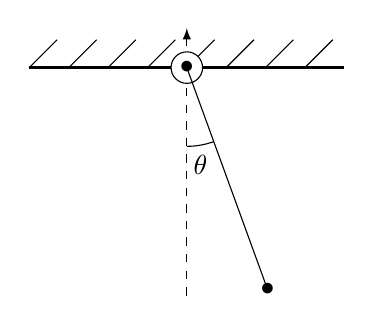
\begin{tikzpicture}
      \draw[decorate,decoration={border,amplitude=0.5cm,segment length=0.5cm}] (-2,0) -- (2,0);
      \draw[dashed,latex-] (0,0.5) -- (0,-3);
      \draw[very thick] (-2,0)-- (2,0);
      \draw[fill=white] (0,0) circle(0.2) node{$\bullet$} -- (-70:3)node{$\bullet$};
      \draw (0,-1) arc (-90:-70:1) node[midway,below]{$\theta$};
    \end{tikzpicture}
    \caption{Pendule simple}
  \end{figure}
  On a la représentation d'état ($x_1=\theta$,$x_2=\dot{\theta}$):
  \[
    \begin{cases}
     \dot{ x_1} = x_2\\
     \dot{x_2} = \frac{-g}{l}sin(x_1)-\frac{k}{m}x_2
    \end{cases}
  \]
Les points d'équilibre vérifient $\dot{x_1}=\dot{x_2} = 0$ soit $x_1= k\pi$,$k\in\Z$. physiquement on a deux points : $0$ et $\pi$.

\item soit le système NL:
  \[
    \begin{cases}

    \dot{x_1}= \alpha + \sin(x_1(t)+x_2(t))+x_1(t)\\
    \dot{x_2}=\alpha+ + \sin(x_1(t)+x_2(t))-x_1(t)
  \end{cases}
\]
Les point d'équilibre sont solutions de $\dot{x_1}=0$ et $\dot{x_2}=0$: on a pas de solution, en effet $\dot{x_1}+\dot{x_2} = 2\alpha+2\sin(x_1+x_2)$ pour $\alpha>1$
\end{enumerate}

\end{exemple}

\begin{rem}
  Les points d'équilibre peuvent aussi être déterminer dans le cas du régime forcé : $\dot{x}(t) = f(\overline{x},\overline{u}) = 0$
\end{rem}

\section{Critère Qualitatif}

\paragraph{But}: Tracer les trajectoires $\chi(t,x_0),\forall x_0\in \D$ dans l'espace de phase $\R^n$ où $n$ est la dimension du système.

Cette méthode est réalisée pour les systèmes du second ordre ,plan de phase dans $\R^2$, voire dans $\R^3$. Les systèmes mécaniques sont des exemples typiques, notamment via les équation de Lagrange $\ddot{q} =l(q,\dot{q})$ avec $q$ coordonnées généralisées. même si le modèle est d'ordre $2n$ où $n = dim(q)$ on peux tracer les coordonnées deux à deux $x_1= q_i ,x_2 = \dot{q_i}$, dans le plan de phase.

\subsection{Méthode pour tracer les trajectoires}
\begin{enumerate}
\item Méthodes informatique :
  \begin{itemize}
  \item   On utlise une intégration numérique pour différentes conditions initiale
  \item Graphe des pentes générés numériquement en étudiant $\deriv[x_1]{x_2} = \frac{f_1(x_1,x_2)}{f_2(x_1,x_2)}$
  \end{itemize}
\item Méthode papier-crayon
  \begin{itemize}
  \item Méthode isocline : peut être manuelle et/ou numérique.
  \item Solution explicite des équations\\
    On élimine le temps de manière explicite ou non.
  \end{itemize}
\end{enumerate}
Dans l'analyse de la stabilité on s'intéresse au comportement dans un voisinage du point d'équilibre.

\begin{defin}
Pour déterminer \emph{l'index topologique} on utilise la méthode suivante:
  \begin{enumerate}
  \item Une courbe autour du point d'équilibre choisie d'une manière arbitraire et supposée de taille infinitésimale
  \item Avec une paramétrisation dans le sens trigonométrique
  \item On considère une suite arbitraire de point $(x_n)$ dans le sens de la paramétrisation
  \item Pour chaque point $x_n$ on évalue $f(x_n$) où $f$  vérifie $\dot{x} =f(x)$.
  \item Tous les vecteurs $f(x_n)_{n=1...N}$ sont ramenés aux point d'équilibre.
  \end{enumerate}
  Ainsi \emph{l'index topologique} est la mesure de l'angle (modulo $2\pi$) que l'extrémité des vecteurs $(f(x_i))$ parcours dans le sens trigonométrique.
\end{defin}
\begin{figure}[ht]
  \centering
    \begin{tikzpicture}
      \node (x) at (0,0) {$\bullet$} node[above]{$\overline{x}$};
      \draw (x) circle (1.5) (20:1.5) node[inputarrow,rotate=110]{};
      \foreach \a in {0,1,2,3,4,5,6,7}
      {\draw[red,-latex] (\a*45:1.5) -- ++(\a*45:0.5);
        \node at (\a*45:2.4){$f(x_\a)$}; }
      \node at (5,0){$\bullet$};
      \foreach \a in {0,1,2,3,4,5,6,7}
      {\draw[red,-latex] (5,0) -- ++(\a*45:0.8);
        \draw (5,0)++(\a*45:1.2)node{$f_\a$}; }
      \node at (5,0){$\bullet$};
      \node[draw,rectangle] at (10,0){index = +1};
    \end{tikzpicture}
    \begin{tikzpicture}
      \node (x) at (0,0) {$\bullet$} node[above]{$\overline{x}$};
      \draw (x) circle (1.5)(20:1.5) node[inputarrow,rotate=110]{};
      \foreach \a/\r in {0/1.2,1/1,2/1,3/1,4/1.2,5/1,6/1,7/1}
      {\draw[red,-latex] (\a*45:1.5) -- ++(-\a*45:0.5);
        \node at (\a*45:\r*2){$f(x_\a)$}; }
      \foreach \a in {0,1,2,3,4,5,6,7}
      {\draw[red,-latex] (5,0) -- ++(-\a*45:0.8);
        \draw (5,0)++(-\a*45:1.2)node{$f_\a$}; }
      \node at (5,0){$\bullet$};
      \node[draw,rectangle] at (10,0){index = -1};
          \end{tikzpicture}

    \begin{tikzpicture}
      \node (x) at (0,0) {$\bullet$} node[above]{$\overline{x}$};
      \draw (x) circle (1.5)(20:1.5) node[inputarrow,rotate=110]{};
      \foreach \a/\t/\r in {0/0/2.5,1/45/2.5,2/0/1.8,3/90/2,4/-45/2,5/45/1.8,6/0/1.8,7/90/2}
      {\draw[red,-latex] (\a*45:1.5) -- ++(\t:0.7);
        \node at (\a*45:\r){$f(x_\a)$}; }
      \foreach \a/\l in {0/137,1/26,2/4,7/5}
      {\draw[red,-latex] (5,0) -- ++(\a*45:0.8);
        \draw (5,0)++(\a*45:1.2)node{$f_{\l}$}; }
      \node at (5,0){$\bullet$};
            \node[draw,rectangle] at (10,0){index = 0};
    \end{tikzpicture}
  \caption{Détermination de l'index topologique}
\end{figure}

Il reste maintenant à chercher les trajectoires autour des points d'équilibres.

\subsection{Méthode isocline}
Pour cette méthode, il s'agit de poser :
\begin{align*}
\frac{dx_2}{dx_1}&= \frac{f_2(x)}{f_1(x)} = Cst \\
\end{align*}
C'est-à-dire de rechercher les points tel que la pente en $x$ est égale à une constante donnée.\\

\begin{exemple}[Pendule inversé]
  Cas sans frottement : \[
    \begin{cases}
    x_1 &= \theta \\
    x_2 &= \dot{\theta}
  \end{cases}
\Rightarrow
\begin{cases}
  x_1 & =x_2\\
  x_2 & = -\frac{g}{l}sin(x_1)
\end{cases}
\]
\smallbreak
Les iso-clines vérifient donc :
\begin{align*}
\frac{dx_2}{dx_1}&= \frac{-\frac{g}{l}sin(x_1)}{x_2}\\
&=C
\intertext{donc les points décrivant la courbe ont pour équation:}
x_2 &= -\frac{g}{lC}sin(x_1)
\end{align*}
On trace alors alors ces courbes pour différentes valeurs de constante et l'on obtient:
\begin{center}
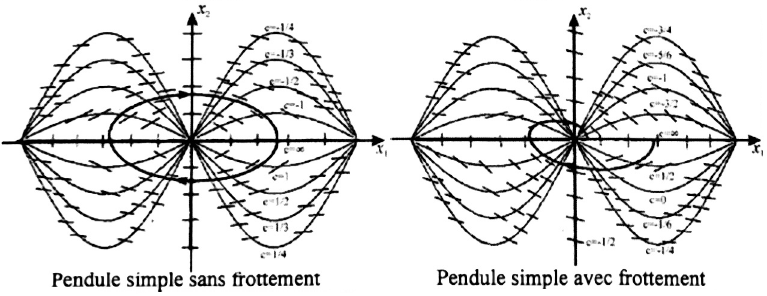
\includegraphics[scale=0.4]{1/graph2.png}
\end{center}


L'iso-cline donne la pente de la trajectoire, ainsi, en suivant les pentes données d'iso-cline en iso-cline, on peut remonter à la trajectoire.\\
A noter que pour $C$ infini on est sur l'axe de $x_1$ et pour $C$ nul sur celui de $x_2$.\\

\begin{rem}
sans frottement on atteint un cycle limite tandis qu'avec frottement on tend bien vers l'origine.
\end{rem}
\end{exemple}

\subsection{Méthode par suppression temporelle}
\subsubsection{Méthode explicite}
À partir des solutions des équations différentielles on se débarasse de la paramétrisation temporelle pour obtenir la trajectoire:
\begin{exemple}
  \[
    \begin{cases}
      \dot{x_1} = x_0 \cos(t) + \dot{x_0} \sin(t)\\
      \dot{x_2} = -x_0 \sin(t) + \dot{x_0} \cos(t)\\
    \end{cases}
  \]
On a $\dot{x_1}^2+\dot{x_2}^2 = x_0^2+\dot{x_0}^2$ soit un cercle de rayon $\sqrt{x_0^2+\dot{x_0}^2}$
\end{exemple}

\subsubsection{Méthode implicite}

Le temps est élimié à partir de l'équation différentielle puis l'orbite est obtenue par intégration
\begin{exemple}
\[
  \begin{cases}
    \dot{x_1}=x_2\\
\dot{x_2} = -x_1
\end{cases}
\implies \frac{\d x_2}{x_2} =\d t = \frac{\d x_1}{x_1}
\]
Donc : \[
  \int_{x_20}^{x_2}x_2\d x_2 = - \int_{x_10}^{x_1}x_1\d x_1
\]
Ainsi on a : $ x_1^2+x_2^2 = x_{10}^2+x_{20}^2$.
\end{exemple}

\begin{rem}
  Les méthodes par élimination du temps ne s'appliquent que pour les systèmes avec des dynamiques relativement simple.
\end{rem}
\end{document}

%%% Local Variables:
%%% mode: latex
%%% TeX-master: "main"
%%% End:
